%%----------------------------------------------------------------------
%%--------------------------------------------------------------
\pagetitle{No Rest for the Weary}

%%----------------------------------------------
%%----------------------------------------------
\begin{columns}

  \emph{No Rest for the Weary} is a minimal two player campaign for
  Recon Squad using the following rules, playing out small actions
  within a larger ongoing battle.

  \missionheading{Campaign}%
  Establish a number of games to play, each a Skirmish or other
  mission.  Recon Squad typically takes~\textasciitilde 90 minutes,
  including setup and cleanup.  The same army lists are used
  throughout.  Players accumulate campaign points from each match as
  follows:

\bigskip\centerline{\fbox{\begin{tabular}{c|cc}
    {\bf Result} & \parbox{2cm}{\centering\bf Victorious} & \parbox[c]{2cm}{\centering\bf Defeated}\\
\hline
\hline
    {\bf Major Victory} & +6 & +0\\
    {\bf Minor Victory} & +4 & +2\\
    {\bf Draw} & +3 & +3\\
\hline
    {\bf Bonus Points} & \multicolumn{2}{c}{+1 for each condition met}
  \end{tabular}}}

%\missionheading{Campaign}%
\bigskip Before each game, the player with the fewest total campaign
points selects which aspect of the larger battle the match will
affect: Reconnaissance, Combat, or Supply Chain.  The first round is
always Combat.  Roll a D3 to determine the aspect if tied.  Track
campaign points earned in each aspect separately.

In addition, after each game both players permanently designate an
additional specialist.  On a major victory the winner designates a
second additional specialist; on a minor victory they do so on a D6
of~4+.  Specialst traits may never repeat in an army.

%\smallskip\missionheading{Battle Hardened}%


%\bigskip
%\vfill%
%\noindent\fbox{\vbox to 3in{(* figure *)}}
%\noindent%
%\begin{minipage}[h]{1.0\linewidth}\centering\small\it%
%\fbox{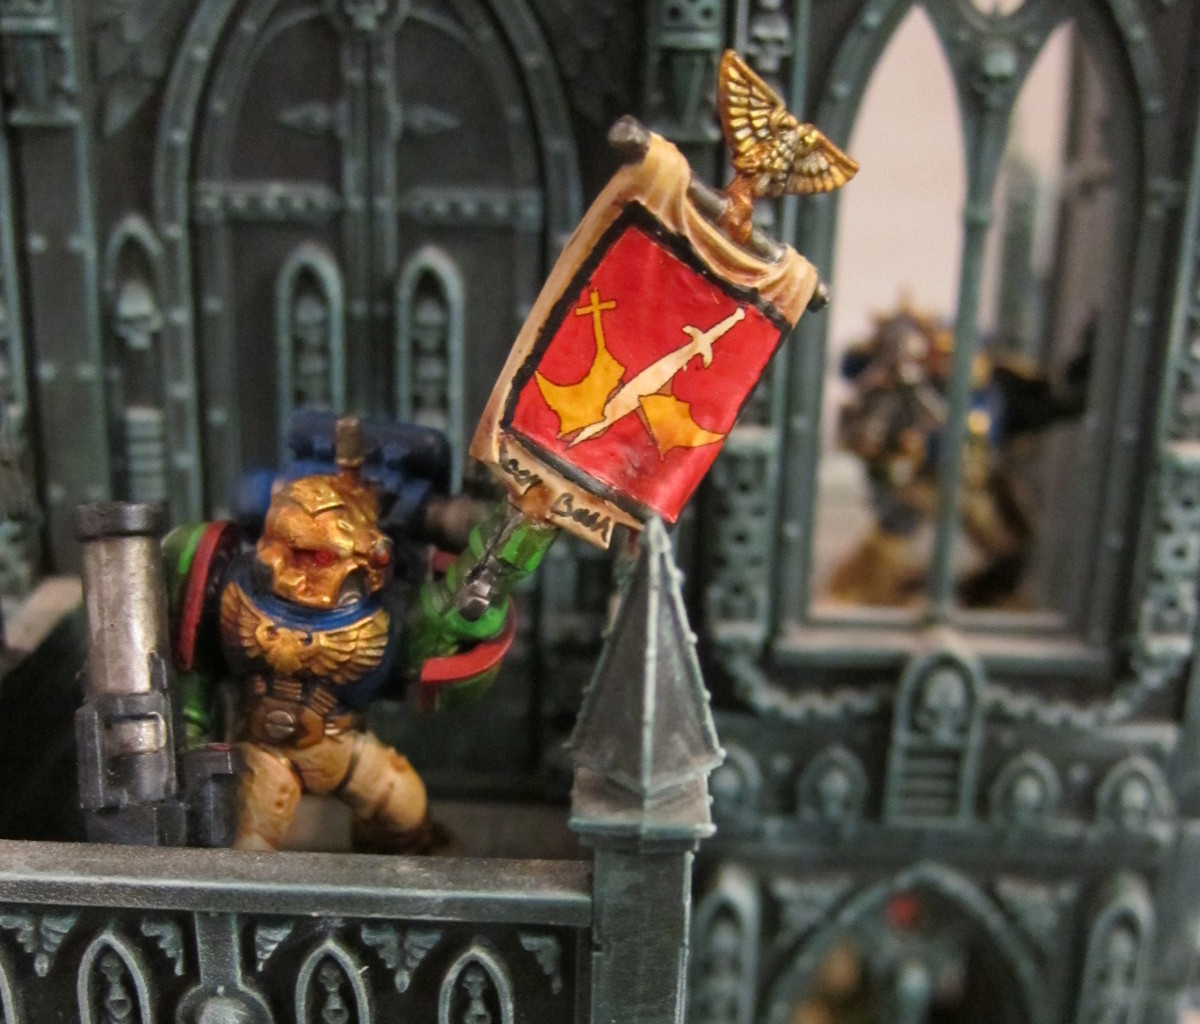
\includegraphics[width=(1.0\linewidth)]{pics/flagbearer-2-cropped}}\\
%From this day forward shall they ever know our name!
%\end{minipage}

%%----------------------------------------------
%%----------------------------------------------
\columnbreak

\begin{sidestory}{0.85in}{War Never-Ending}%
  Hulgurth swept ponderously back and forth, his chainsword idling
  wildly.  Finding no foes in reach on which to slake his bloodthirst,
  he vented his frustration by crushing in the side of the smoking
  troop carrier next to him with the heel of his fist.  Bellowing in
  rage, he began loping heavily, hungrily after the quickly retreating
  figures in the distance.  This was not over.  This would never be
  over.
\end{sidestory}

If a player has no more non-specialist, non-vehicle models to
designate, they may give an additional trait to an existing
specialist.  Models may not be given a third trait until all
specialists have two, and so on.

%Clearly record which models have which traits.  It may be useful to
%subtly but clearly mark their bases.

\missionheading{Victory!}%

At the campaign's end a player wins by either:

\vspace*{-4pt}
\begin{itemize}
\item Having the most campaign points in Combat and one other
  aspect---\emph{a strategic victory!}

\vspace*{-4pt}
\item Or, having twice as many Combat campaign points as their
  opponent---\emph{brute conquest!}
\end{itemize}
\vspace*{-4pt}

If neither condition is met, the battle grinds on in interminable
stalemate---\emph{there can be only war!!!}


\end{columns}%

\vfill
\hrule
\smallskip
\hrule

\begin{multicols}{2}
%%----------------------------------------------
\missionheading{Disclaimer}%

Recon Squad is completely unofficial, unauthorized, and unaffiliated
with Games Workshop.

\smallskip{\footnotesize Adepta Sororitas, Adeptus Astartes, Astra
  Militarum, Blood Angels, Chaos Daemons, Chaos Space Marines, Dark
  Angels, Dark Eldar, Eldar, Grey Knights, Necrons, Orks, Space
  Wolves, Tau Empire, Tyranid, Forge World, Games Workshop, Warhammer,
  and all associated marks, names, races, race insignia, characters,
  vehicles, locations, units, illustrations, images, and models from
  the Warhammer 40,000 universe and game are either \textregistered,
  TM, and/or \textcopyright\ Copyright Games Workshop Ltd 2000--2014.
  Used without permission, no challenge to status intended, all rights
  reserved to their respective owners.}

% variably registered in the UK and other countries.

% All Games Workshop marks and terms have been used without
% permission; no challenge to their status is intended.  All rights
% are reserved to their respective owners.

\vfill
\vbox to 0 pt{}

%%----------------------------------------------
\columnbreak
\missionheading{Credits}%

\smallskip\noindent {\bf Design:}
\begin{minipage}[t]{3in}
The Philadelphia Area Gaming Enthusiasts\\
\centerline{\url{http://pagegaming.com/}}
\end{minipage}

\smallskip\noindent{\bf Text, Photos, and Typesetting:} Joe Kopena

\smallskip\noindent{\bf Cover Art:} Luke Walker

\smallskip\noindent This PDF has been produced using solely open source
tools: Emacs, \LaTeX, Inkscape, and GIMP.

%%----------------------------------------------
\missionheading{Version}%

\noindent This is \emph{Recon Squad} \today.

\vspace*{0.5in}\hbox to 0pt{}
\end{multicols}%

\begin{tikzpicture}[remember picture, overlay]%
    \node[inner sep=0pt,above left,xshift=1.75cm,yshift=1.7cm] at (current page.south east) {%
        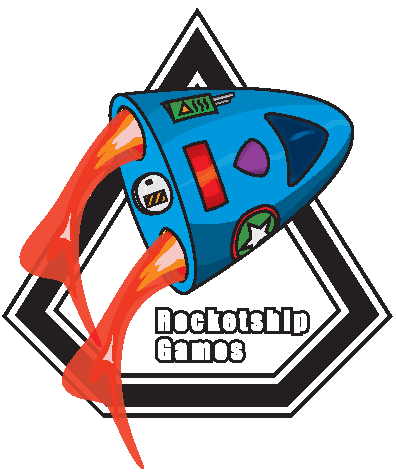
\includegraphics[width=1.5in]{art/rocketshipgames-logo}%
    };%
\end{tikzpicture}

%\begin{tikzpicture}[remember picture, overlay]
%  \draw [fill=white,draw=none] (current page.south west) rectangle (2,0.25) ;%
%\end{tikzpicture}

\begin{tikzpicture}[remember picture, overlay]
  \node[above=72pt,xshift=1in,draw=none,text centered] at (current page.south) {%
    \scalebox{2}{{\sf\Large\bf rocketshipgames.com}}%
  };%
\end{tikzpicture}

%%%%%\pagetitle{
%\vfill
%\centerline{%
%\noindent\centerline{\scalebox{2}{{\sf\Large\bf rocketshipgames.com}}}%
%}
%\hfill
%\raisebox{-0.5\height}[0pt][0pt]{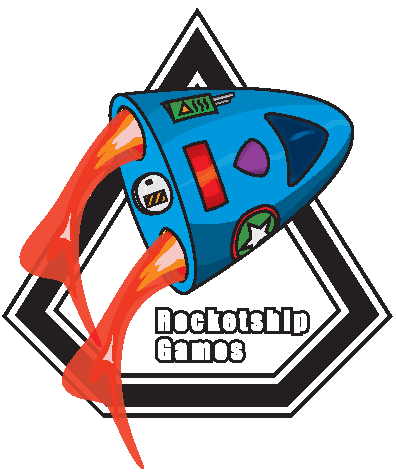
\includegraphics[width=1.5in]{art/rocketshipgames-logo}}%
